\documentclass[11pt]{article}

\usepackage[margin=1in]{geometry}
\usepackage{amsmath,amssymb,amsthm}
\usepackage{mathtools}
\usepackage{graphicx}
\usepackage{booktabs}
\usepackage{xcolor}
\usepackage[numbers,sort&compress]{natbib}
\usepackage[colorlinks=true,linkcolor=blue!50!black,citecolor=blue!50!black,urlcolor=blue!50!black]{hyperref}
\usepackage[capitalize]{cleveref}

\newtheorem{proposition}{Proposition}
\newtheorem{corollary}{Corollary}
\theoremstyle{definition}
\newtheorem{definition}{Definition}
\newtheorem{assumption}{Assumption}
\theoremstyle{remark}
\newtheorem{remark}{Remark}

% Draft markers; remove before submission.
\newcommand{\todo}[1]{\textcolor{red}{[TODO: #1]}}

\newcommand{\clip}{\operatorname{clip}}
\newcommand{\val}[2]{\langle #1\rangle_{#2}}
\newcommand{\hLP}{h^{\mathrm{LP}}}

\title{Square-Root Perpetuals from Concentrated Liquidity:\\
Range Rolling, Out-of-Range Residuals, and Funding}
\author{Shuhei Hiya\thanks{Teliha, Inc. Email: \texttt{syuhei176@gmail.com}.}}
\date{October 22, 2026}

\begin{document}
\maketitle

\begin{abstract}
A full-range constant-product liquidity position with liquidity $L$ is worth $2L\sqrt{x}$ and replicates a perpetual on the square root of the price $x$. Concentrated liquidity, as in Uniswap~v3, has this shape only inside a price range. We show that a concentrated position with liquidity $L$ on $[a,b]$, held together with a \emph{static account} of $L/\sqrt{b}$ units of token0 and $L\sqrt{a}$ units of token1, holds exactly the token amounts of a full-range position whenever $a\le x\le b$, and those of the full-range position at the nearest boundary otherwise. Based on this identity we give a range-rolling rule. A roll performed while the price is inside both the old and the new range moves a price-independent amount of tokens between the pool and the static account, needs no swap and no price oracle, and preserves delta and gamma. A roll performed after the price has left the range leaves a residual whose value is exactly $V\,(\cosh(u/2)-1)\ge 0$, where $V$ is the position value and $u$ the log-distance past the boundary; the residual is second order in $u$ while the swap that clears it is first order. The theoretical funding rate of the resulting perpetual is $\sigma^2 V/8$, consistent with loss-versus-rebalancing and earlier results on $0.5$-power perpetuals. Simulations quantify roll frequency and residuals. On-chain data from the Predy protocol on Arbitrum confirm the residual formula: the cost of clearing late-roll residuals equalled the pool fee plus a small price impact, and no late roll had a negative net surplus. On the pools of Predy V5 in 2023--2024, fee-linked funding reached between 64\% and 94\% of realized $\sigma^2/8$.
\end{abstract}

\section{Introduction}

Power perpetuals pay a funding stream for exposure to a power of an index price without expiry~\cite{white2021power}. For the power $1/2$ there is a natural on-chain replicating portfolio: a position in a constant-product market maker (CPMM) with liquidity $L$ is worth $2L\sqrt{x}$ when the pool price is $x$~\cite{clark2020replicating}. Robinson, Clark and Leone~\cite{robinson2024perp} make this explicit, describing CPMMs as replicating portfolios of a $0.5$-power perpetual and relating its funding to the equilibrium fee rate $\sigma^2/8$. For concentrated liquidity they only note that ``the extension to Uniswap v3 is straightforward and left to the reader.''

The extension is the subject of this paper. Concentrated liquidity~\cite{adams2021uniswap} lets a liquidity provider (LP) supply liquidity $L$ only on a price interval $[a,b]$. Inside the interval the position behaves like a full-range position with the same $L$; outside it holds only one token and has no curvature. A concentrated position on its own therefore behaves like a fixed-strike option position~\cite{lambert2022panoptic}, not like $\sqrt{x}$. To keep $\sqrt{x}$ exposure as the price moves, the interval has to be moved (\emph{rolled}). Rolling burns the old position and mints a new one. In general this produces surplus tokens and requires swaps, and the exposure changes during the roll. The questions are whether rolling can be made exact, swap-free and oracle-free, and what happens when a roll is late.

\paragraph{Contributions.}
\begin{enumerate}
  \item \emph{Static construction} (\cref{prop:static}). A concentrated position with liquidity $L$ on $[a,b]$ plus a static account $S(a,b)=(L/\sqrt{b},\,L\sqrt{a})$ holds the token amounts $F(x)=(L/\sqrt{x},\,L\sqrt{x})$ of a full-range position inside the range and $F(c)$ outside, where $c$ is the nearest boundary. Only a fraction $1-e^{-h/2}\approx h/2$ of the value sits in the pool for a range of log-half-width $h$; the rest is plain tokens.
  \item \emph{Range rolling} (\cref{prop:roll}). A roll inside the range moves exactly $S(a',b')-S(a,b)$ between the pool and the static account. This amount does not depend on the price, so no swap or oracle is needed, and the total holdings, delta and gamma are unchanged.
  \item \emph{Out-of-range residual} (\cref{prop:residual,cor:cost}). A late roll leaves a residual $F(c)-F(x)$ worth $V(\cosh(u/2)-1)\approx Vu^2/8\ge 0$. Clearing it requires a swap of notional $\tfrac{V}{2}|e^{u/2}-1|\approx V|u|/4$, so with a pool fee $\varphi$ the residual pays for its own swap once $|u|\gtrsim 2\varphi$. We discuss who should receive the residual.
  \item \emph{Funding} (\cref{prop:funding}). Under geometric Brownian motion the fair funding received by the long side is $\sigma^2V/8$, which matches the loss-versus-rebalancing (LVR) rate of a CPMM~\cite{milionis2022lvr} and the $0.5$-power perpetual result of~\cite{robinson2024perp}. Pool fees accrue per unit of in-range liquidity, so fee growth is an oracle-free funding index for a position of size $L$.
  \item \emph{Implementation, simulation and on-chain evidence.} The construction underlies the Squart perpetual of the Predy protocol~\cite{predy2023sqrt,predy2024c4} (\cref{sec:predy}). Simulations (\cref{sec:sim}) confirm the propositions to machine precision and quantify roll frequency and residuals as functions of range width and monitoring interval. Events from Predy V5 and V6 on Arbitrum One (\cref{sec:onchain}) show that roll frequencies follow~\eqref{eq:roll-rate}, that the residuals of late rolls cleared at the pool fee as predicted by \cref{cor:cost}, and that fee-linked funding came close to $\sigma^2/8$ on the main ETH pool.
\end{enumerate}

The construction was first written up by the author in February 2023~\cite{hiya2023note}. It has been used in production since Predy V3.2 launched on Arbitrum in March 2023, and this paper gives its formal treatment.

\section{Related work}\label{sec:related}

\paragraph{Replication by AMMs and power perpetuals.}
Clark~\cite{clark2020replicating} derives the replicating portfolio of a CPMM, and~\cite{clark2021bounded} treats bounded liquidity. Power perpetuals were introduced in~\cite{white2021power} with emphasis on powers greater than one; \cite{robinson2024perp} discusses the $0.5$-power perpetual and its relation to full-range CPMMs. Angeris, Evans and Chitra~\cite{angeris2022monotonic} show that monotonic payoffs can be replicated without oracles by designing the trading function of a constant function market maker. We instead keep the existing Uniswap~v3 trading function and obtain the target payoff by adding a static account and a rolling rule.

\paragraph{Liquidity positions as options and borrowed liquidity.}
Panoptic~\cite{lambert2022panoptic} treats fixed-range Uniswap~v3 positions as perpetual options and obtains long option exposure by borrowing liquidity. GammaSwap~\cite{gammaswap} lets traders borrow full-range CPMM liquidity, which gives short $\sqrt{x}$ exposure on v2-style pools. InfinityPools~\cite{infinitypools} borrows concentrated liquidity to obtain leveraged linear exposure. In these designs the range of a given position is fixed, or the pool is full-range. Here the range is rolled so that the exposure is $\sqrt{x}$ at all prices while the liquidity stays concentrated.

\paragraph{Impermanent loss, pricing and hedging.}
Fukasawa, Maire and Wunsch~\cite{fukasawa2023weighted} hedge the impermanent loss of CPMMs with weighted variance swaps. Deng, Zong and Wang~\cite{deng2023static} statically replicate the impermanent loss of concentrated positions with options. Lipton, Lucic and Sepp~\cite{lipton2024unified} decompose funded and borrowed Uniswap~v2/v3 positions into vanilla, digital and square-root payoffs for a fixed range. Maire and Wunsch~\cite{maire2024market} construct market-neutral concentrated positions with options and futures, and Hou, Yu and Xu~\cite{hou2024risk} price v3 positions with a stopping-time approach. These works price or hedge a given position. We synthesize a target payoff from positions whose range changes over time. LVR~\cite{milionis2022lvr} gives the arbitrage cost of providing liquidity and, for a CPMM, coincides with the funding rate derived in \cref{sec:funding}.

\paragraph{Leverage and position management.}
Elsts and Klas~\cite{elsts2024leverage} model margin and debt for leveraged concentrated liquidity. Vlasov, Gorgadze and Barger~\cite{vlasov2025framework} give a framework for moving positions to new ranges. Strategic range choice is studied in~\cite{neuder2021strategic,fan2022differential}. Our rolling rule is specific in that it keeps the total holdings, rather than the LP position alone, invariant.

\section{Preliminaries}\label{sec:prelim}

Consider a pool of token0 (the risky asset, e.g.\ ETH) and token1 (the numeraire, e.g.\ USDC), and let $x>0$ be the pool price of token0 in units of token1. A \emph{holding} is a vector $h=(h^0,h^1)\in\mathbb{R}^2$ of token amounts; negative entries are debts. Its value at price $x$ is
\[
  \val{h}{x} = x\,h^0 + h^1 .
\]

\begin{definition}[Concentrated position]
A Uniswap~v3 position with liquidity $L>0$ on the range $[a,b]$, $0<a<b$, holds~\cite{adams2021uniswap}
\begin{equation}\label{eq:lp}
  \hLP(x;a,b) = \Bigl(L\bigl(\tfrac{1}{\sqrt{c}}-\tfrac{1}{\sqrt{b}}\bigr),\; L\bigl(\sqrt{c}-\sqrt{a}\bigr)\Bigr),
  \qquad c=\clip(x;a,b)\coloneqq\min\{\max\{x,a\},b\}.
\end{equation}
Inside the range its value is $\val{\hLP}{x}=L\bigl(2\sqrt{x}-\sqrt{a}-x/\sqrt{b}\bigr)$.
\end{definition}

Letting $a\to 0$ and $b\to\infty$ gives the \emph{full-range holdings}
\begin{equation}\label{eq:full}
  F(x) = \bigl(L/\sqrt{x},\; L\sqrt{x}\bigr),\qquad \val{F(x)}{x} = 2L\sqrt{x}.
\end{equation}
We write $V(x)=2L\sqrt{x}$ for the target value. Since $V$ is concave, every tangent of $V$ lies above it.

\begin{assumption}\label{ass:frictionless}
(i) Positions can be minted and burned at the current pool price $x$; pool fees earned and gas costs are ignored in \cref{sec:static,sec:roll}. (ii) Tokens can be held, deposited in a lending market as collateral, or borrowed against collateral; interest is ignored unless stated. (iii) When stated, swaps execute at price $x$ with a proportional fee $\varphi$ on the notional.
\end{assumption}

\section{Static construction}\label{sec:static}

\begin{definition}[Static account]
For a range $[a,b]$ and liquidity $L$, the static account is
\[
  S(a,b) = \bigl(L/\sqrt{b},\; L\sqrt{a}\bigr).
\]
\end{definition}

\begin{proposition}[Static construction]\label{prop:static}
For every $x>0$,
\[
  \hLP(x;a,b) + S(a,b) = F\bigl(\clip(x;a,b)\bigr).
\]
In particular, the combined position has value $V(x)=2L\sqrt{x}$ for $x\in[a,b]$, and value $L\bigl(x/\sqrt{c}+\sqrt{c}\bigr)$ outside the range, which is the tangent of $V$ at the nearest boundary $c\in\{a,b\}$.
\end{proposition}

\begin{proof}
Adding $S(a,b)$ to~\eqref{eq:lp} gives $\bigl(L/\sqrt{c},\,L\sqrt{c}\bigr)=F(c)$. Its value at $x$ is $L(x/\sqrt{c}+\sqrt{c}) = V(c)+V'(c)(x-c)$.
\end{proof}

\begin{corollary}[Greeks]\label{cor:greeks}
Inside the range the combined position has $\Delta = L/\sqrt{x}$ and $\Gamma = -L/(2x^{3/2})$, the same as a full-range position with liquidity $L$. Outside the range $\Delta = L/\sqrt{c}$ and $\Gamma=0$, and the value exceeds $V(x)$.
\end{corollary}

\Cref{fig:payoff} illustrates the construction. Two features are worth noting.

First, the static account has non-negative entries, so an unlevered long $\sqrt{x}$ position requires no borrowing. Leverage is obtained by borrowing token1 against the position. A long perpetual of size $L$ opened at $x_0$ holds $\hLP+S$ and owes $V(x_0)$ of token1; while the price stays inside the range its profit and loss is $2L(\sqrt{x}-\sqrt{x_0})$. A short position is the mirror image: it borrows the liquidity $L$ (and the static account) and sells it.

Second, most of the value is held outside the pool. For a range centred at the current price in log terms, $a=xe^{-h}$ and $b=xe^{h}$,
\begin{equation}\label{eq:pool-share}
  \frac{\val{\hLP}{x}}{V(x)} = 1-e^{-h/2} \approx \frac{h}{2},
\end{equation}
so for $h=5\%$ only about $2.5\%$ of the position value is in the pool. The static account consists of plain tokens that can be deposited in a lending market and used as collateral or lent out.

\begin{figure}[t]
  \centering
  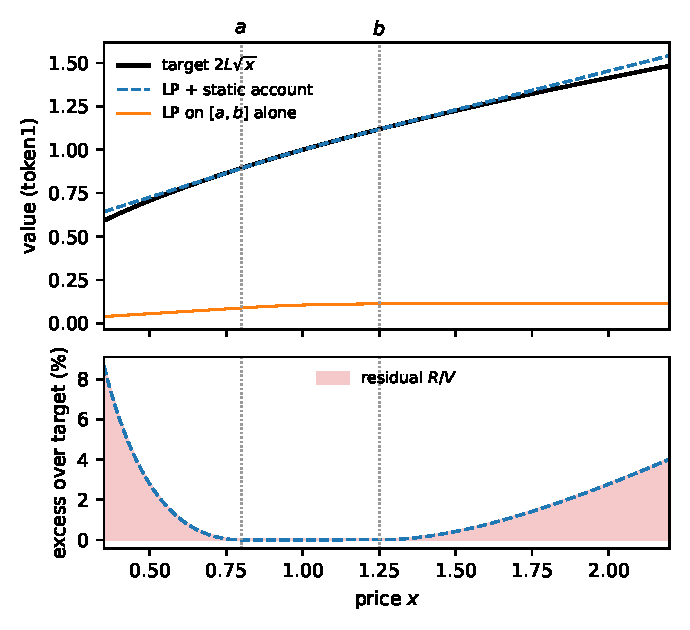
\includegraphics[width=0.62\linewidth]{figures/payoff.pdf}
  \caption{Top: value of a concentrated position on $[a,b]=[0.8,1.25]$ alone, of the position plus static account (\cref{prop:static}), and of the target $2L\sqrt{x}$ ($L=1/2$). Bottom: excess of the combined position over the target. It is zero inside the range; outside, the combined position follows the tangent at the boundary and the shaded excess is the residual of \cref{prop:residual}.}
  \label{fig:payoff}
\end{figure}

\section{Range rolling}\label{sec:roll}

A \emph{roll} from $[a,b]$ to $[a',b']$ at price $x$ burns the position $\hLP(\cdot;a,b)$, mints $\hLP(\cdot;a',b')$ with the same liquidity $L$, and transfers the tokens released (or required) to (or from) the static account.

\begin{proposition}[In-range roll]\label{prop:roll}
If $x\in[a,b]\cap[a',b']$, the tokens released by the roll are
\[
  \hLP(x;a,b)-\hLP(x;a',b') = S(a',b')-S(a,b)
  = \Bigl(L\bigl(\tfrac{1}{\sqrt{b'}}-\tfrac{1}{\sqrt{b}}\bigr),\; L\bigl(\sqrt{a'}-\sqrt{a}\bigr)\Bigr),
\]
which does not depend on $x$. After the transfer the position is exactly $\hLP(\cdot;a',b')+S(a',b')$. Its holdings remain $F(x)$, and its delta and gamma are unchanged.
\end{proposition}

\begin{proof}
By \cref{prop:static}, $\hLP(x;a,b)+S(a,b)=F(x)=\hLP(x;a',b')+S(a',b')$ when $x$ lies in both ranges. Rearranging gives the first identity. Greeks follow from \cref{cor:greeks}, since they depend only on $L$ and $x$ inside the range.
\end{proof}

When the range moves up ($a'\ge a$, $b'\ge b$), token0 leaves the static account and token1 enters it; when it moves down, the reverse. A fully funded static account always covers the tokens the mint requires: moving up needs $L(1/\sqrt{b}-1/\sqrt{b'})\le L/\sqrt{b}=S^0(a,b)$ of token0, and moving down needs $L(\sqrt{a}-\sqrt{a'})\le L\sqrt{a}=S^1(a,b)$ of token1. After a sequence of in-range rolls through $[a_k,b_k]$, $k=0,\dots,n$, the increments telescope and the account is $S(a_n,b_n)$ regardless of the path. In an implementation that does not hold $S$ per position, the increments are booked as deposits and debts in a lending pool (\cref{sec:predy}).

Rolls are needed only near the boundaries. With a range re-centred at each roll, $[xe^{-h},xe^{h}]$, and a roll triggered when the log-distance to a boundary falls below $\theta<h$, the log-price must travel $h-\theta$ between rolls. For volatility $\sigma$ the expected exit time of a Brownian motion from an interval of half-width $d$ is $d^2/\sigma^2$, so the number of rolls per unit time is approximately
\begin{equation}\label{eq:roll-rate}
  \frac{\sigma^2}{(h-\theta)^2}.
\end{equation}

\subsection{Out-of-range rolls}

On a blockchain a roll happens at discrete times, and the price may leave the range before the next roll.

\begin{proposition}[Out-of-range residual]\label{prop:residual}
Let $x\notin[a,b]$, $c=\clip(x;a,b)\in\{a,b\}$, and $x\in[a',b']$. After the roll the position holds $\hLP(x;a',b')+S(a',b')+r$, with residual
\[
  r = F(c)-F(x) = \Bigl(L\bigl(\tfrac{1}{\sqrt{c}}-\tfrac{1}{\sqrt{x}}\bigr),\; L\bigl(\sqrt{c}-\sqrt{x}\bigr)\Bigr).
\]
The two entries of $r$ have opposite signs, and the value of the residual is
\begin{equation}\label{eq:residual}
  R \coloneqq \val{r}{x} = \frac{L(\sqrt{x}-\sqrt{c})^2}{\sqrt{c}}
    = V(x)\bigl(\cosh(u/2)-1\bigr) \ge 0,\qquad u=\ln(x/c).
\end{equation}
Swapping the token0 entry of $r$ at price $x$ restores the holdings $F(x)$ and leaves a surplus of $R$ units of token1.
\end{proposition}

\begin{proof}
Burning and minting only move tokens between the pool and the account, so the total holdings just before and after the roll are both $F(c)$ by \cref{prop:static}. The target after the roll is $\hLP(x;a',b')+S(a',b')=F(x)$, again by \cref{prop:static}. The difference is $r$. Its value is $L(x/\sqrt{c}+\sqrt{c}-2\sqrt{x}) = L(\sqrt{x}-\sqrt{c})^2/\sqrt{c}$. With $s=\sqrt{x/c}=e^{u/2}$, $R/V(x)=(s-1)^2/(2s)=(s+s^{-1})/2-1=\cosh(u/2)-1$.
\end{proof}

The residual has a simple interpretation. Between leaving the range at $c$ and the roll at $x$, the position keeps the boundary delta $L/\sqrt{c}$ instead of the target delta $L/\sqrt{y}$, and
\[
  R = \int_c^x \Bigl(\frac{L}{\sqrt{c}}-\frac{L}{\sqrt{y}}\Bigr)\,dy .
\]
Equivalently, it is the gamma the position did not pay while it was out of range.

\begin{corollary}[Swap cost]\label{cor:cost}
The swap that clears the residual has notional $x|r^0| = \tfrac{1}{2}V(x)\,|e^{u/2}-1|$ in token1. With a proportional fee $\varphi$, the net surplus is
\[
  V(x)\Bigl(\cosh(u/2)-1-\tfrac{\varphi}{2}\,|e^{u/2}-1|\Bigr)
  = V(x)\Bigl(\tfrac{u^2}{8}-\tfrac{\varphi|u|}{4}\Bigr)+O(|u|^3),
\]
which is positive for $|u|\gtrsim 2\varphi$. For a $5$\,bp pool this is an overshoot of about $0.1\%$.
\end{corollary}

\begin{remark}[Who receives the residual]\label{rem:allocation}
The residual is non-negative and can be assigned in several ways. (i) Credited to the position holders: the product then pays the tangent instead of $2L\sqrt{x}$ during excursions and dominates the target. This is the choice made in Predy V5 (\cref{sec:predy}). (ii) Paid to whoever executes the roll: the reward grows quadratically in the overshoot, so a permissionless keeper rolls once the reward exceeds its execution cost. This is the choice made in Predy V6. (iii) Accumulated in a protocol reserve. Under (ii) and (iii) the holders receive exactly $2L\sqrt{x}$ at every roll.
\end{remark}

\section{Funding}\label{sec:funding}

\begin{proposition}[Theoretical funding]\label{prop:funding}
Let $dx_t=\sigma x_t\,dW_t$ with token1 as numeraire and zero interest rates. Then $V(x)=2L\sqrt{x}$ satisfies
\[
  dV_t = \Delta_t\,dx_t - \frac{\sigma^2}{8}\,V_t\,dt,\qquad \Delta_t=L/\sqrt{x_t},
\]
and $\mathbb{E}[V_T]=V_0\,e^{-\sigma^2T/8}$. A long position that receives funding at rate $f_t=\sigma^2V_t/8$ and is delta-hedged has zero expected profit.
\end{proposition}

\begin{proof}
By It\^o's formula, $dV = V'(x)\,dx + \tfrac12 V''(x)\sigma^2x^2\,dt$ with $V'=L/\sqrt{x}$ and $V''=-\tfrac12 Lx^{-3/2}$, so the drift is $-\tfrac14 L\sigma^2\sqrt{x}=-\tfrac{\sigma^2}{8}V$. Taking expectations gives $d\,\mathbb{E}[V_t]=-\tfrac{\sigma^2}{8}\mathbb{E}[V_t]\,dt$.
\end{proof}

Because $\sqrt{x}$ is concave, the long side is short gamma and must be paid to hold the position, just as a liquidity provider is paid fees. The rate $\sigma^2V/8$ equals the instantaneous LVR of a CPMM with value $V$~\cite{milionis2022lvr} and the equilibrium funding of a $0.5$-power perpetual in~\cite{robinson2024perp}. By \cref{cor:greeks} the rolled construction has exactly this gamma while it is in range. While it is out of range its gamma is zero, and the gamma not paid is returned as the residual $R$ at the next roll (\cref{prop:residual}).

In practice the funding can be tied to realized pool fees instead of an estimate of $\sigma$. Uniswap~v3 distributes fees pro rata over in-range liquidity, so a concentrated position with liquidity $L$ earns, while in range, the same fees as a full-range position with liquidity $L$ would earn at the same active liquidity. The fee growth inside the current range is therefore a natural, oracle-free funding index for a $\sqrt{x}$ perpetual of size $L$. Whether realized fees track $\sigma^2V/8$ depends on the balance of arbitrage and noise trading in the pool~\cite{milionis2022lvr}.

\section{Implementation in Predy}\label{sec:predy}

Predy offers a perpetual called Squart, indexed to $\sqrt{x}$, by supplying and borrowing Uniswap~v3 liquidity. We describe two versions deployed on Arbitrum One: V5, whose Controller contract was deployed in July 2023~\cite{predy2023sqrt}, and V6, deployed in January 2024 and audited in May 2024~\cite{predy2024c4}. Both implement the construction of \cref{sec:static,sec:roll} in the same way and differ in how the out-of-range residual is settled.

\paragraph{Pooled position and rolling.} For each pair the protocol holds one Uniswap~v3 position. Liquidity is supplied by users who are long $\sqrt{x}$ and borrowed by users who are short. A permissionless \texttt{reallocate} function rolls the range when the current tick is within a threshold number of ticks $\theta$ of either boundary, or outside the range. It burns the whole position and mints the same liquidity on a new range $[\text{tick}-h,\ \text{tick}+h]$ around the current tick, rounded to the tick spacing. The difference between the tokens received and the tokens required is booked as a deposit or a debt in the protocol's lending pools (the \emph{rebalance position}); these are the increments of \cref{prop:roll}. Interest on the rebalance position is distributed per unit of Squart. When the lending pool cannot supply the token required, the new range is shifted less far.

\paragraph{Out-of-range rolls.} If the price is outside the range, the contract computes the residual of \cref{prop:residual} at the crossed boundary. In V5 the contract swaps the token0 leg of the residual in the same Uniswap pool and records the remaining token1 balance as \texttt{profit}. A positive profit is credited to the suppliers as additional fee growth, which is option~(i) of \cref{rem:allocation}; a negative profit has to be paid by the caller. In V6 the caller settles the token0 leg through an external swap supplied in a settlement callback, and any surplus of the quote token is transferred to the caller. This is option~(ii): the keeper receives $R$ net of its execution cost.

\paragraph{Funding.} In both versions funding is tied to pool fees. Per unit of borrowed liquidity, the short side pays the fee growth inside the range multiplied by $1+s(U)$, where $U$ is the utilization (borrowed over supplied liquidity) and
\[
  s(U) = 1.6\,\bigl(\max\{U-0.1,\,0\}\bigr)^2 .
\]
Suppliers receive the fee growth multiplied by $1+U\,s(U)$.

\section{Numerical experiments}\label{sec:sim}

\paragraph{Setup.} We simulate $x_t$ as a geometric Brownian motion with $\sigma=80\%$ per year and zero rates, starting at $x_0=1$ with $L=1/2$ so that $V_0=1$. The range is re-centred at each roll, $[xe^{-h},xe^{h}]$, and a roll is triggered when the log-distance to a boundary falls below $\theta=h/5$. The trigger is checked only every $\Delta t$, which models block time and keeper latency. We vary $h\in\{2,5,10,20\}\%$ and $\Delta t\in\{1\text{ min},10\text{ min},1\text{ h},1\text{ day}\}$, and run 400 paths of one year for each pair. Token holdings are tracked explicitly through every burn, mint, transfer and swap, not through the closed forms; the residual swap is charged a $5$\,bp fee. Code and data are available at \url{https://github.com/syuhei176/portfolio/tree/main/papers/sqrt-perp}.

\paragraph{Checks.} Over all runs, the largest absolute deviation from \cref{prop:static} and \cref{prop:roll} was $0$ in floating point, and the largest deviation of $R/V$ from $\cosh(u/2)-1$ was $2.4\times10^{-16}$. A Monte Carlo estimate of $\mathbb{E}[\sqrt{x_1}]$ from $2\times10^6$ samples was $0.92325\pm0.00027$, against $e^{-\sigma^2/8}=0.92312$ from \cref{prop:funding}.

\begin{figure}[t]
  \centering
  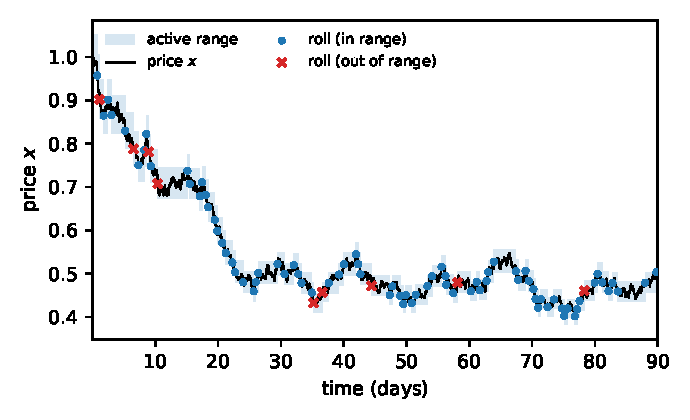
\includegraphics[width=0.62\linewidth]{figures/path.pdf}
  \caption{One simulated path over 90 days ($h=5\%$, $\theta=1\%$, hourly checks). The shaded band is the active range; dots mark rolls inside the range and crosses mark rolls after the price had left it.}
  \label{fig:path}
\end{figure}

\begin{table}[t]
  \centering
  \small
  \begin{tabular}{llrrrrrr}
\toprule
$\Delta t$ & $h$ & rolls/yr & $\sigma^2/(h-\theta)^2$ & out-of-range & $\sum R/V$ & swap notional & net of 5\,bp \\
 & & & & share & (\%/yr) & ($\times V$/yr) & (\%/yr) \\
\midrule
1 min & 2\% & 2309 & 2500 & 0.0\% & 0.000 & 0.000 & 0.000 \\
1 min & 5\% & 387 & 400 & 0.0\% & 0.000 & 0.000 & 0.000 \\
1 min & 10\% & 98 & 100 & 0.0\% & 0.000 & 0.000 & 0.000 \\
1 min & 20\% & 25 & 25 & 0.0\% & 0.000 & 0.000 & 0.000 \\
\addlinespace
10 min & 2\% & 1947 & 2500 & 13.4\% & 0.012 & 0.095 & 0.008 \\
10 min & 5\% & 360 & 400 & 0.1\% & 0.000 & 0.000 & 0.000 \\
10 min & 10\% & 95 & 100 & 0.0\% & 0.000 & 0.000 & 0.000 \\
10 min & 20\% & 25 & 25 & 0.0\% & 0.000 & 0.000 & 0.000 \\
\addlinespace
1 h & 2\% & 1396 & 2500 & 48.5\% & 0.281 & 0.732 & 0.244 \\
1 h & 5\% & 312 & 400 & 12.8\% & 0.011 & 0.035 & 0.010 \\
1 h & 10\% & 88 & 100 & 0.7\% & 0.000 & 0.000 & 0.000 \\
1 h & 20\% & 23 & 25 & 0.0\% & 0.000 & 0.000 & 0.000 \\
\addlinespace
1 day & 2\% & 257 & 2500 & 90.2\% & 3.623 & 1.594 & 3.543 \\
1 day & 5\% & 138 & 400 & 71.7\% & 1.138 & 0.569 & 1.110 \\
1 day & 10\% & 56 & 100 & 48.1\% & 0.275 & 0.145 & 0.267 \\
1 day & 20\% & 18 & 25 & 20.0\% & 0.028 & 0.017 & 0.027 \\
\bottomrule
\end{tabular}

  \caption{Rolls and residuals over one year ($\sigma=80\%$, $\theta=h/5$, mean of 400 paths). ``Out-of-range share'' is the fraction of rolls that happened after the price had left the range. $\sum R/V$ is the total residual relative to the position value at each roll; the theoretical funding for comparison is $\sigma^2/8=8\%$ per year. ``Net of 5\,bp'' subtracts the fee on the residual swap.}
  \label{tab:rolls}
\end{table}

\paragraph{Results.} \Cref{fig:path} shows a sample path and \cref{tab:rolls} summarizes the grid. The number of rolls follows~\eqref{eq:roll-rate} closely when monitoring is frequent and falls below it when monitoring is coarse, because several crossings are merged into one roll. With checks every minute, fewer than $0.01\%$ of rolls happened out of range, since a move larger than $\theta$ within one minute is very unlikely at this volatility. Residuals become material only when the monitoring interval is long compared with the time needed to cross the threshold. With daily checks and $h=2\%$, $90\%$ of rolls were late and the residual added up to $3.6\%$ of the position value per year, almost half of the theoretical funding of $8\%$. With hourly checks and $h\ge 5\%$ the residual was below $0.02\%$ per year. \Cref{fig:residual} shows that individual residuals follow \cref{prop:residual} and that, in line with \cref{cor:cost}, the $5$\,bp swap cost exceeds the residual only for overshoots below about $0.1\%$.

\begin{figure}[t]
  \centering
  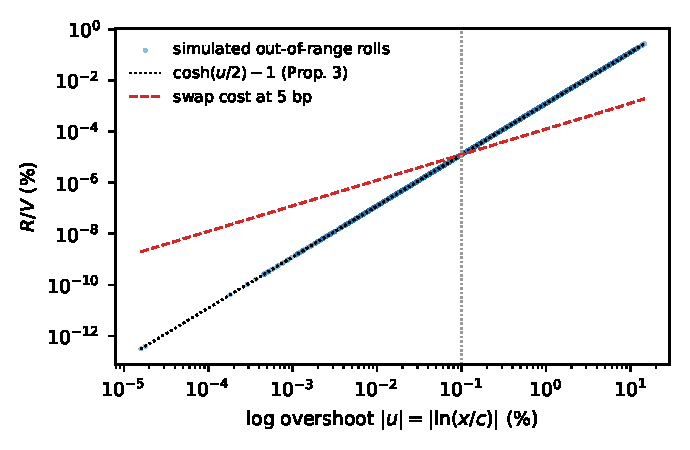
\includegraphics[width=0.62\linewidth]{figures/residual.pdf}
  \caption{Residual relative to position value against the log-overshoot $|u|$ for simulated out-of-range rolls (hourly and daily checks, log--log scale), with the exact curve of \cref{prop:residual} (slope 2) and the swap cost of \cref{cor:cost} at $5$\,bp (slope 1). The curves cross at $|u|\approx 2\varphi=0.1\%$ (dotted line).}
  \label{fig:residual}
\end{figure}

\section{On-chain evidence}\label{sec:onchain}

\paragraph{Data.} We collected all \texttt{Rebalanced} and \texttt{PremiumGrowthUpdated} events emitted by the V5 Controller (\texttt{0x06a6\ldots9829}) and the V6 PredyPool (\texttt{0x9215\ldots8613}) on Arbitrum One up to block 517{,}138{,}812 (October 2026) from a public RPC endpoint, together with hourly prices from Binance for realized variance. V5 performed 1{,}574 rolls on 10 of its 14 pairs, most of them between July 2023 and February 2024. In V6, Squart liquidity was supplied only from April 18 to May 14, 2024, and only 4 rolls took place, none out of range; the analysis below therefore relies mainly on V5. Scripts and the derived data are part of the replication package.

\paragraph{Roll frequency.} \Cref{tab:onchain} lists the pairs with at least 20 rolls. For volatile pairs the observed number of rolls per year is between $0.67$ and $1.11$ times the prediction~\eqref{eq:roll-rate} computed from realized volatility over the same period. This is in line with \cref{sec:sim}: rolls are triggered by keepers at discrete times, and several threshold crossings can be merged into one roll.

\begin{table}[t]
  \centering
  \scriptsize
  \begin{tabular}{llrrrrrr}
\toprule
pair (pool fee) & period & $(h,\theta)$ & rolls & rolls/yr & $\sigma^2/(h-\theta)^2$ & out of range & median $|u|$ \\
 & & (ticks) & & & & (share) & (out of range) \\
\midrule
V5 WETH/USDC.e (5\,bp) & 2023-07-13--2024-05-18 & (720, 360) & 160 & 189 & 215 & 3 (1.9\%) & 1.24\% \\
V5 ARB/USDC.e (30\,bp) & 2023-07-06--2024-05-17 & (720, 360) & 418 & 483 & 669 & 3 (0.7\%) & 2.09\% \\
V5 GYEN/USDC.e (5\,bp) & 2023-08-11--2024-05-06 & (120, 60) & 30 & 41 & -- & 1 (3.3\%) & 1.13\% \\
V5 LUSD/USDC.e (5\,bp) & 2023-07-15--2024-02-08 & (60, 30) & 52 & 91 & -- & 1 (1.9\%) & 0.65\% \\
V5 WETH/USDC.e (5\,bp) & 2023-07-05--2024-02-13 & (190, 70) & 540 & 883 & 1316 & 21 (3.9\%) & 0.46\% \\
V5 WETH/USDC (5\,bp) & 2023-07-13--2023-11-09 & (720, 360) & 33 & 101 & 108 & 0 (0.0\%) & -- \\
V5 ARB/USDC (5\,bp) & 2023-07-06--2023-12-22 & (720, 360) & 155 & 336 & 434 & 1 (0.6\%) & 0.19\% \\
V5 WBTC/WETH (5\,bp) & 2023-09-29--2024-01-09 & (480, 240) & 46 & 165 & 148 & 1 (2.2\%) & 0.79\% \\
V5 ARB/WETH (5\,bp) & 2023-07-14--2023-12-12 & (480, 240) & 123 & 297 & 410 & 0 (0.0\%) & -- \\
\bottomrule
\end{tabular}

  \caption{Rolls of Predy V5 on Arbitrum One for pairs with at least 20 rolls. $h$ and $\theta$ are the range half-width and roll threshold in ticks ($1\text{ tick}\approx 0.01\%$). The prediction $\sigma^2/(h-\theta)^2$ uses realized volatility from hourly Binance prices over the period shown; it is not available for stablecoin pairs.}
  \label{tab:onchain}
\end{table}

\paragraph{Out-of-range rolls and residuals.} 31 of the 1{,}574 V5 rolls ($2.0\%$) happened after the price had left the range. For each of them the transaction receipt contains the Uniswap swap that cleared the residual, which gives the token0 leg $r^0$ exactly, and the recorded profit gives the token1 leg $r^1$. \Cref{prop:residual} implies $-r^1/r^0=\sqrt{cx}$, so the price at the roll is recovered as $x=(r^1/r^0)^2/c$. In all 31 cases this price lies outside the previous range on the side of the crossed boundary, and in 27 cases it lies within 10 ticks of the centre of the new range, which the contract sets from the current tick (in the other four the new range was not centred on the roll price). The log-overshoot had median $|u|=0.61\%$, 90th percentile $3.7\%$ and maximum $4.9\%$. \Cref{fig:onchain-residual} compares the residual with the realized profit. The difference between them is the cost of the residual swap. Relative to the pool fee times the swap notional, this cost had median $1.02$ and 10th to 90th percentiles $1.00$ to $1.12$, so the cost was essentially the pool fee plus a small price impact, as assumed in \cref{cor:cost}. No out-of-range roll had a negative net profit. For the USD-quoted pairs, residuals of $\$920$ in total yielded $\$878$ of net profit, which was credited to the suppliers.

\begin{figure}[t]
  \centering
  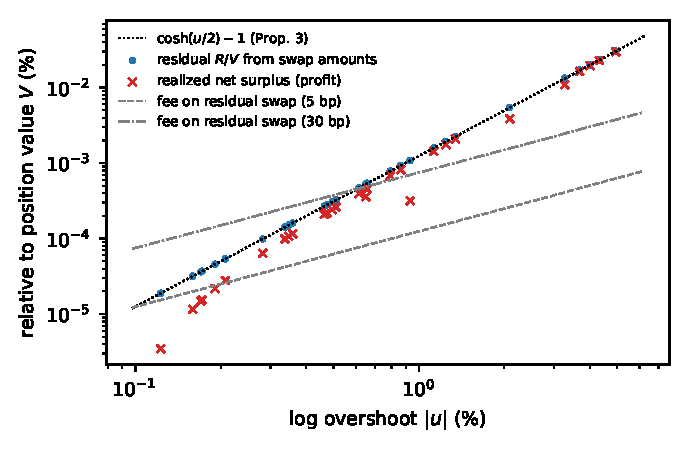
\includegraphics[width=0.62\linewidth]{figures/onchain_residual.pdf}
  \caption{The 31 out-of-range rolls of Predy V5. Dots: residual value recovered from the swap amounts via \cref{prop:residual}; crosses: realized net profit recorded by the contract. Dashed lines: pool fee on the residual swap from \cref{cor:cost} for 5 and 30\,bp pools.}
  \label{fig:onchain-residual}
\end{figure}

\paragraph{Fee-linked funding.} For each month in which a USD-quoted pair held at least $\$10{,}000$ of Squart, we sum the fee growth reported by \texttt{PremiumGrowthUpdated}, convert it into fees per unit of position value $V=2L\sqrt{x}$ using the hourly price, and annualize. \Cref{fig:onchain-funding} plots it against realized $\sigma^2/8$ for the same month, and \cref{tab:funding} aggregates by pair. On the bridged-USDC ETH pool with a $\pm720$-tick range, fees amounted to $0.94$ of $\sigma^2/8$ over eight months, close to the equilibrium value of \cref{prop:funding}. The same pool with a narrower $\pm190$-tick range captured $0.80$, consistent with the narrower range spending more time out of range, where it earns no fees. The ARB pool with a 30\,bp fee captured $0.81$, the native-USDC ETH pool $0.64$ in 2023, and V6 on the native-USDC pool only $0.17$ in its two months. Utilization was low throughout, so the spread $s(U)$ added at most $3.5\%$ to the funding paid by the short side.

\begin{figure}[t]
  \centering
  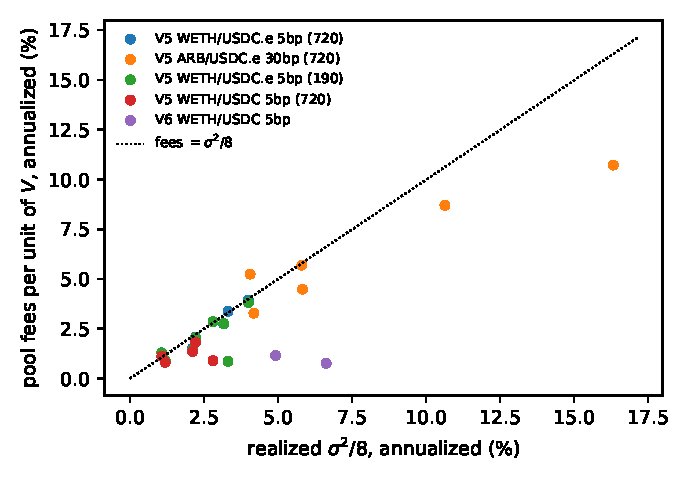
\includegraphics[width=0.62\linewidth]{figures/onchain_funding.pdf}
  \caption{Monthly pool fees earned per unit of position value against realized $\sigma^2/8$, annualized, for USD-quoted Predy pairs with at least $\$10{,}000$ of Squart in the month. The dotted line is equality, the theoretical funding of \cref{prop:funding}. Range half-widths in ticks are given in parentheses.}
  \label{fig:onchain-funding}
\end{figure}

\begin{table}[t]
  \centering
  \small
  \begin{tabular}{llrrrr}
\toprule
version, pair & pool fee & months & $\sum$ fees / $\sum \sigma^2/8$ & mean $U$ & premium uplift \\
\midrule
V5, WETH/USDC.e & 5\,bp & 8 & 0.94 & 0.17 & 3.5\% \\
V5, ARB/USDC.e & 30\,bp & 6 & 0.81 & 0.06 & 1.3\% \\
V5, WETH/USDC.e & 5\,bp & 8 & 0.80 & 0.12 & 3.4\% \\
V5, WETH/USDC & 5\,bp & 5 & 0.64 & 0.00 & 0.0\% \\
V6, WETH/USDC & 5\,bp & 2 & 0.17 & 0.00 & 0.0\% \\
\bottomrule
\end{tabular}

  \caption{Fee-linked funding against realized variance by pair. ``Premium uplift'' is the additional funding paid by the short side through $s(U)$.}
  \label{tab:funding}
\end{table}

\section{Discussion and limitations}\label{sec:discussion}

\paragraph{Frictions.} The invariants ignore pool fees, gas and interest. Pool fees earned by the position add to the long side's income and are the basis of fee-linked funding. Gas makes very narrow ranges expensive, since by~\eqref{eq:roll-rate} the number of rolls grows like $h^{-2}$. Interest on the static account and on any debt changes the carry but not the payoff identities.

\paragraph{Tick discretization.} Ranges are restricted to multiples of the tick spacing. \Cref{prop:static,prop:roll,prop:residual} hold for arbitrary $a<b$ and $a'<b'$, so discretization does not break exactness. It only changes where the boundaries are.

\paragraph{Price manipulation.} Rolls are executed at the pool price. An attacker who pushes the price past a boundary can force an out-of-range roll. If the residual is paid to the executor, the attacker would collect it. The residual is second order in the push while the cost of moving the pool is first order, but the residual scales with the size of the perpetual position while the cost scales with pool depth. Safe parameters therefore depend on the ratio of the two, and time-weighted prices can be used for checks.

\paragraph{Discrete monitoring and jumps.} \Cref{tab:rolls} shows that late rolls, rather than the construction itself, are the main source of deviation from $2L\sqrt{x}$. Jumps across the threshold within one block cannot be avoided by monitoring alone; the residual formula bounds their effect.

\section{Conclusion}

A concentrated liquidity position plus a static account of $L/\sqrt{b}$ token0 and $L\sqrt{a}$ token1 holds the full-range amounts $(L/\sqrt{x},L\sqrt{x})$ inside its range. Rolling the range moves a price-independent amount of tokens between the pool and the account, with no swap and no oracle. Late rolls leave a non-negative residual $V(\cosh(u/2)-1)$ that can pay for its own clearing. Together with fee-linked funding this gives an exact, oracle-free construction of a $\sqrt{x}$ perpetual from Uniswap~v3, the extension left open in~\cite{robinson2024perp}. Data from the Predy deployment on Arbitrum agree with the residual formula and its swap cost, and show fee-linked funding between $0.64$ and $0.94$ of realized $\sigma^2/8$ on the V5 pools. Why the ratio varies across pools and periods, and in particular why it was low on the native-USDC pool in 2024, is left for future work.

\bibliographystyle{plainnat}
\bibliography{refs}

\end{document}
